\documentclass{ximera}

%\colorlet{penColor}{blue!50!black} % Color of a curve in a plot
%\colorlet{gridColor}{gray!50} % Color of grid in a plot
%\colorlet{background}{white} % Color of the page
\newcommand{\ddx}{\frac{d}{dx}}
\newcommand{\dydx}{\frac{dy}{dx}}
\newcommand{\dd}[2][]{\frac{d #1}{d #2}}



\outcome{Understand the relationship between the graph of a function and the graph of its derivative.}
\outcome{Understand the relationship between differentiability and continuity.}
\outcome{Estimate the slope of the tangent line graphically.}
\outcome{Graph the derivative function.}
\outcome{Determine whether a piecewise function is differentiable.}


\title{Introduction to derivatives}

\begin{document}

\begin{abstract}
  The derivative gives a formula for the slope of the tangent line of a curve.
\end{abstract}
\maketitle


Suppose that $f(x)$ is a function.  It is often useful to know how
sensitive the value of $f(x)$ is to small changes in $x$. To give you
a feeling why this is true, consider the following:
\begin{itemize}
\item If $p(t)$ represents the position of an object with respect to
  time, the rate of change gives the velocity of the object.
\item If $v(t)$ represents the velocity of an object with respect to
  time, the rate of change gives the acceleration of the object.
\item The rate of change of a function can help us approximate a
  complicated function with a simple function.
\item The rate of change of a function can be used to help us solve
  equations that we would not be able to solve via other methods.
\end{itemize}

The rate of change of a function is the slope of the tangent line. For
now, consider the following informal definition of a \textit{tangent
  line}:
\begin{quote}
Given a function $f(x)$, if one can ``zoom in''
on $f(x)$ sufficiently so that $f(x)$ seems to be a straight line,
then that line is the \textbf{tangent line} to $f(x)$ at the point
determined by $x$.
\end{quote}
We illustrate this informal definition with the following picture:

\begin{image}
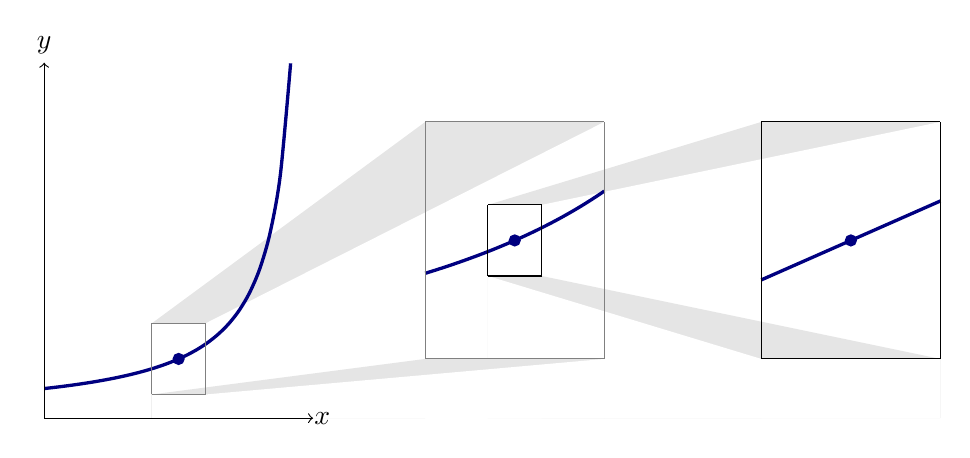
\begin{tikzpicture}
\colorlet{penColor}{blue!50!black}
%\colorlet{penColor2}{red!50!black}
	\begin{axis}[
            domain=0:6, range=0:7,
            ymin=-.2,ymax=7,
            width=6in,
            height=7cm, %% Hard coded height! Moreover this effects the aspect ratio of the zoom--sort of BAD
            axis lines=none,
          ]   
          \addplot [draw=none, fill=black!10!white] plot coordinates {(.8,1.6) (2.834,5)} \closedcycle; %% zoom fill
          \addplot [draw=none, fill=black!10!white] plot coordinates {(2.834,5) (4.166,5)} \closedcycle; %% zoom fill
          \addplot [draw=none, fill=white] plot coordinates {(1.2,1.6) (4.166,5)} \closedcycle; %% zoom fill
          \addplot [draw=none, fill=white] plot coordinates {(.8,1.6) (1.2,1.6)} \closedcycle; %% zoom fill

          \addplot [draw=none, fill=black!10!white] plot coordinates {(3.3,3.6) (5.334,5)} \closedcycle; %% zoom fill
          \addplot [draw=none, fill=black!10!white] plot coordinates {(5.334,5) (6.666,5)} \closedcycle; %% zoom fill
          \addplot [draw=none, fill=white] plot coordinates {(3.7,3.6) (6.666,5)} \closedcycle; %% zoom fill
          \addplot [draw=none, fill=white] plot coordinates {(3.3,3.6) (3.7,3.6)} \closedcycle; %% zoom fill
          
          \addplot [draw=none, fill=black!10!white] plot coordinates {(3.7,2.4) (6.666,1)} \closedcycle; %% zoom fill
          \addplot [draw=none, fill=black!10!white] plot coordinates {(3.3,2.4) (3.7,2.4)} \closedcycle; %% zoom fill
          \addplot [draw=none, fill=white] plot coordinates {(3.3,2.4) (5.334,1)} \closedcycle; %% zoom fill          
          \addplot [draw=none, fill=white] plot coordinates {(5.334,1) (6.666,1)} \closedcycle; %% zoom fill
          

          \addplot [draw=none, fill=black!10!white] plot coordinates {(.8,.4) (2.834,1)} \closedcycle; %% zoom fill
          \addplot [draw=none, fill=black!10!white] plot coordinates {(2.834,1) (4.166,1)} \closedcycle; %% zoom fill
          \addplot [draw=none, fill=white] plot coordinates {(1.2,.4) (4.166,1)} \closedcycle; %% zoom fill
          \addplot [draw=none, fill=white] plot coordinates {(.8,.4) (1.2,.4)} \closedcycle; %% zoom fill

          \addplot[very thick,penColor, smooth,domain=(0:1.833)] {-1/(x-2)};
          \addplot[very thick,penColor, smooth,domain=(2.834:4.166)] {3.333/(2.050-.3*x)-0.333}; %% 2.5 to 4.333
          %\addplot[very thick,penColor, smooth,domain=(5.334:6.666)] {11.11/(1.540-.09*x)-8.109}; %% 5 to 6.833
          \addplot[very thick,penColor, smooth,domain=(5.334:6.666)] {x-3}; %% 5 to 6.833
          
          \addplot[color=penColor,fill=penColor,only marks,mark=*] coordinates{(1,1)};  %% point to be zoomed
          \addplot[color=penColor,fill=penColor,only marks,mark=*] coordinates{(3.5,3)};  %% zoomed pt 1
          \addplot[color=penColor,fill=penColor,only marks,mark=*] coordinates{(6,3)};  %% zoomed pt 2

          \addplot [->,black] plot coordinates {(0,0) (0,6)}; %% axis
          \addplot [->,black] plot coordinates {(0,0) (2,0)}; %% axis
          
          \addplot [black!50!white] plot coordinates {(.8,.4) (.8,1.6)}; %% box around pt
          \addplot [black!50!white] plot coordinates {(1.2,.4) (1.2,1.6)}; %% box around pt
          \addplot [black!50!white] plot coordinates {(.8,1.6) (1.2,1.6)}; %% box around pt
          \addplot [black!50!white] plot coordinates {(.8,.4) (1.2,.4)}; %% box around pt
          
          \addplot [black!50!white] plot coordinates {(2.834,1) (2.834,5)}; %% zoomed box 1
          \addplot [black!50!white] plot coordinates {(4.166,1) (4.166,5)}; %% zoomed box 1
          \addplot [black!50!white] plot coordinates {(2.834,1) (4.166,1)}; %% zoomed box 1
          \addplot [black!50!white] plot coordinates {(2.834,5) (4.166,5)}; %% zoomed box 1

          \addplot [black] plot coordinates {(3.3,2.4) (3.3,3.6)}; %% box around zoomed pt
          \addplot [black] plot coordinates {(3.7,2.4) (3.7,3.6)}; %% box around zoomed pt
          \addplot [black] plot coordinates {(3.3,3.6) (3.7,3.6)}; %% box around zoomed pt
          \addplot [black] plot coordinates {(3.3,2.4) (3.7,2.4)}; %% box around zoomed pt

          \addplot [black] plot coordinates {(5.334,1) (5.334,5)}; %% zoomed box 2
          \addplot [black] plot coordinates {(6.666,1) (6.666,5)}; %% zoomed box 2
          \addplot [black] plot coordinates {(5.334,1) (6.666,1)}; %% zoomed box 2
          \addplot [black] plot coordinates {(5.334,5) (6.666,5)}; %% zoomed box 2

          \node at (axis cs:2.2,0) [anchor=east] {$x$};
          \node at (axis cs:0,6.6) [anchor=north] {$y$};
        \end{axis}
\end{tikzpicture}
\end{image}


The \textit{derivative} of a function $f(x)$ at $x$, is the slope of
the tangent line at $x$. To find the slope of this line, we consider
\textit{secant} lines, lines that locally intersect the curve at two
points.  The slope of any secant line that passes through the points
$(x,f(x))$ and $(x+h, f(x+h))$ is given by

\[
\frac{\Delta y}{\Delta x}=\frac{f(x+h) -f(x)}{(x+h)-x} = \frac{f(x+h)-f(x)}{h}.
\]

See the following picture:


\begin{image}
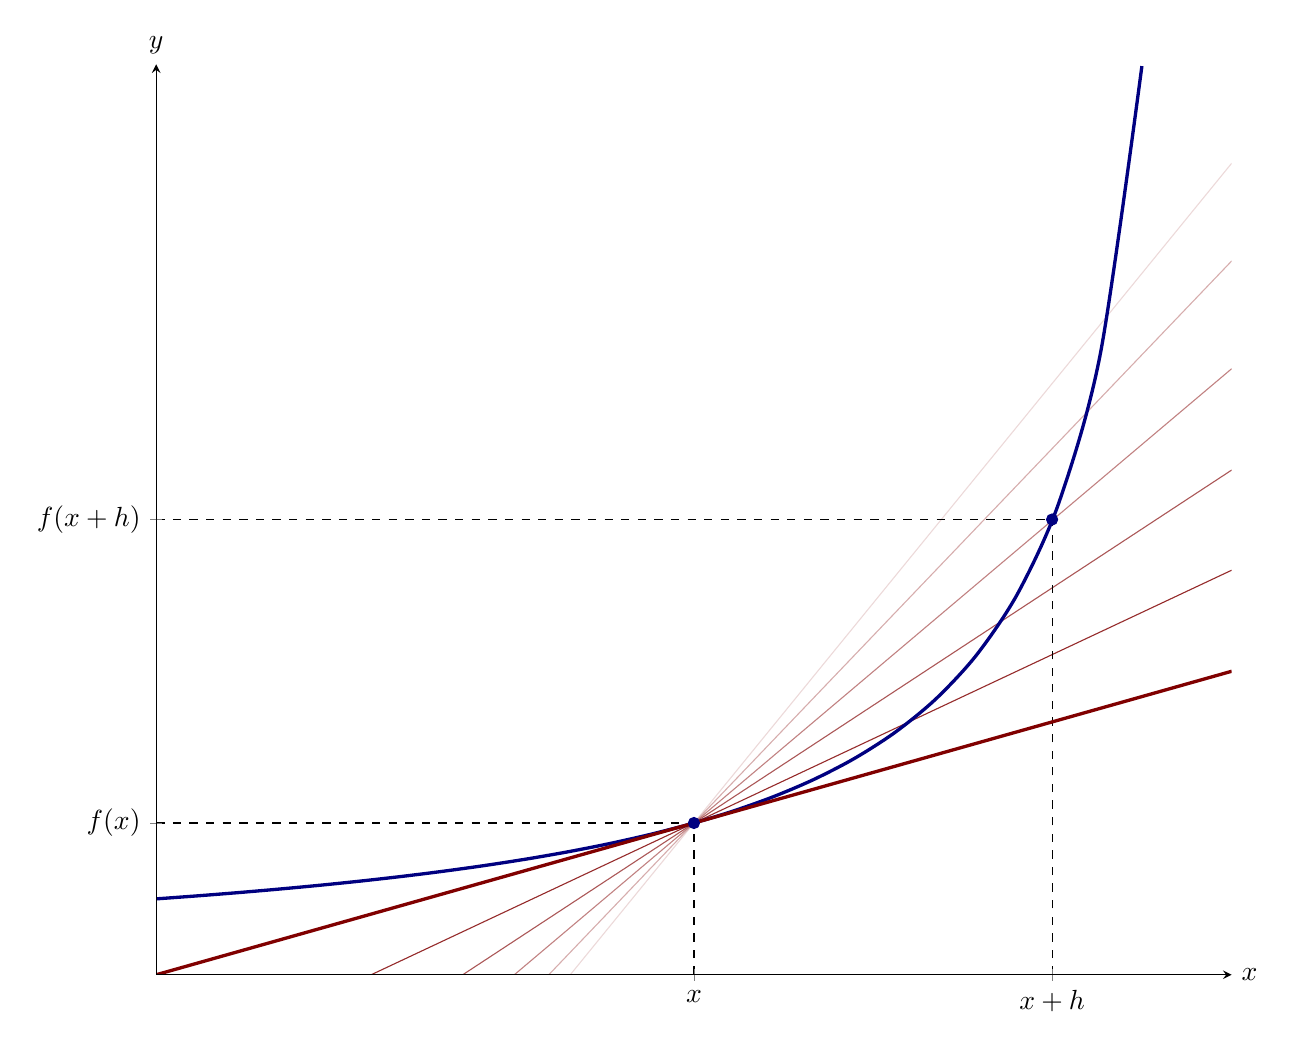
\begin{tikzpicture}
\colorlet{penColor}{blue!50!black}
\colorlet{penColor2}{red!50!black}
	\begin{axis}[
            domain=0:2, range=0:6,ymax=6,ymin=0,
            width=6in,
            axis lines =left, xlabel=$x$, ylabel=$y$,
            every axis y label/.style={at=(current axis.above origin),anchor=south},
            every axis x label/.style={at=(current axis.right of origin),anchor=west},
            xtick={1,1.666}, ytick={1,3},
            xticklabels={$x$,$x+h$}, yticklabels={$f(x)$,$f(x+h)$},
            axis on top,
          ]         
          \addplot [penColor2!15!white, domain=(0:2)] {-3.348+4.348*x};
          \addplot [penColor2!32!white, domain=(0:2)] {-2.704+3.704*x};
          \addplot [penColor2!49!white, domain=(0:2)] {-1.994+2.994*x};         
          \addplot [penColor2!66!white, domain=(0:2)] {-1.326+2.326*x}; 
          \addplot [penColor2!83!white, domain=(0:2)] {-0.666+1.666*x};
	  \addplot [black,dashed] plot coordinates {(1,0) (1,1)};
          \addplot [black,dashed] plot coordinates {(0,1) (1,1)};
          \addplot [black,dashed] plot coordinates {(0,3) (1.666,3)};
          \addplot [black,dashed] plot coordinates {(1.666,0) (1.666,3)};
          \addplot [very thick,penColor, smooth,domain=(0:1.833)] {-1/(x-2)};
          \addplot[color=penColor,fill=penColor,only marks,mark=*] coordinates{(1.666,3)};  %% closed hole          
          \addplot[color=penColor,fill=penColor,only marks,mark=*] coordinates{(1,1)};  %% closed hole          
          \addplot [very thick,penColor2, smooth,domain=(0:2)] {x};
        \end{axis}
\end{tikzpicture}
\end{image}
This leads to the \textit{limit definition of the derivative}:


\begin{definition}
The \textbf{derivative} of $f(x)$ is the function

\[
\ddx f(x) = \lim_{h\to 0} \frac{f(x+h) - f(x)}{h}.
\]

If this limit does not exist for a given value of $x$, then $f(x)$ is
not \textbf{differentiable} at $x$.
\end{definition}

\begin{question}
  What is the difference between a ``derivative'' and ``slope''?
    \begin{multipleChoice}
      \choice[correct]{All of these.}
      \choice{A derivative is defined as a limit, while slope is simply a ratio of numbers.}
      \choice{A derivative is a function that tells the slope of the tangent line at different points.}
      \choice{A slope is always constant, while a derivative is a function (which could be constant).}
    \end{multipleChoice}  
\end{question}

\begin{definition}
There are several different notations for the derivative, we'll mainly
use
\[
\ddx f(x) = f'(x).
\]
If one is working with a function of a variable other than $x$, say $t$ we write
\[
\dd{t} f(t) = f'(t).
\]
However, if $y = f(x)$, $\dydx$, $\dot{y}$, and $D_x f(x)$ are
also used.
\end{definition}

\begin{question}
  Given $f(x) = 3x+7$, what is $f'(x)$?
    \begin{multipleChoice}
      \choice[correct]{$3$}
      \choice{$3x+7$}
      \choice{$7$}
      \choice{Impossible to determine.}
    \end{multipleChoice}  
\end{question}


\begin{question}
  The following computation is computing the derivative of some
  function $f(x)$ at some point $a$:

\[
\lim_{h\to 0} \frac{\sqrt{5+h}-\sqrt{5}}{h}
\]
Which of the following below could be $f(x)$? Which could be $a$?
    \begin{multipleChoice}
      \choice[correct]{$f(x) = \sqrt{x}$, $a=5$.}
      \choice{$f(x) = \sqrt{5+h}$, $a=5$.}
      \choice{$f(x) = \frac{\sqrt{5+h}-\sqrt{5}}{h}$, $a=0$.}
      \choice{$f(x) = \sqrt{x}$, $a=h$.}
    \end{multipleChoice}  
\end{question}


\begin{question}
  Let $f(x) = e^\pi$. What is $f'(x)$?
  \begin{hint}
    What does a plot of $e^\pi$ look like?
  \end{hint}
    \begin{multipleChoice}
      \choice[correct]{$0$}
      \choice{$e^\pi$}
      \choice{$\pi\cdot e^{\pi-1}$}
      \choice{$\pi\cdot e^{\pi}$}
    \end{multipleChoice}  
\end{question}



\begin{question}
Write down at least \textbf{five} questions for this lecture. After
you have your questions, label them as ``Level 1,'' ``Level 2,'' or ``Level 3'' where:
\begin{description}
\item[Level 1] Means you know the answer, or know exactly how to do this problem.
\item[Level 2] Means you think you know how to do the problem, or will soon learn how to do the problem.
\item[Level 3] Means you have no idea how to do the problem. 
\end{description}
  \begin{freeResponse}
  \end{freeResponse}
\end{question}

\end{document}
